\documentclass{article}
\usepackage{tikz, calc}
\usepackage{comment}
\usetikzlibrary{positioning}

\definecolor{myyellow}{RGB}{255,255,150}

\newcommand\mytext[3][\scriptsize]{#2\\#1 #3}
\newcommand\mynode[4][]{%
  \node[mynode,#1,text width=\the\dimexpr#2cm*3] (#3) {\mytext{#3}{#2 #4}}; 
}

\begin{document}

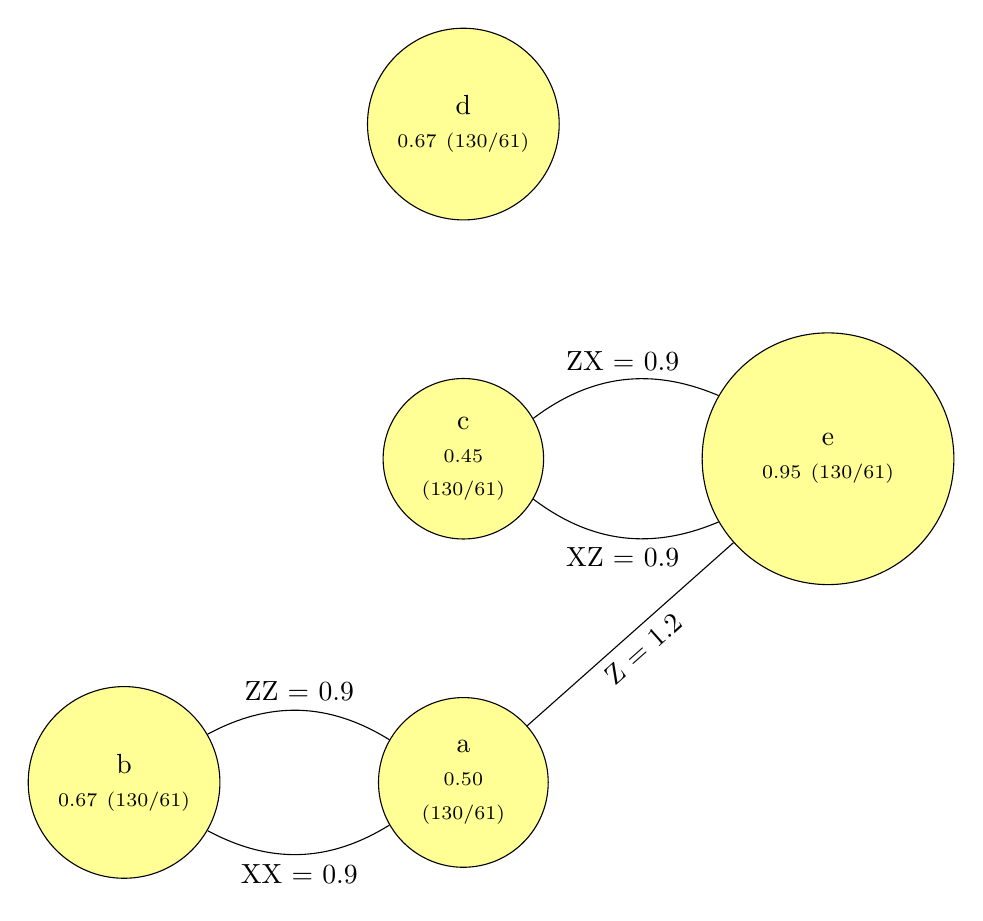
\begin{tikzpicture}[
node distance=2cm,
mynode/.style={
  circle,
  draw,
  fill=myyellow,
  align=center}
]

\mynode{0.67}{d}{(130/61)}
\mynode[below=of d]{0.45}{c}{(130/61)}
\mynode[below=of c]{0.50}{a}{(130/61)} 
\mynode[left=of a]{0.67}{b}{(130/61)} 
\mynode[right=of c]{0.95}{e}{(130/61)}

\begin{comment}
\draw[-] 
  (d) -- node[rotate=90,below] {\mytext[\normalsize]{XX =}{0.9}} (c); 
\draw[-] 
  (c) -- node[rotate=90,below] {\mytext[\normalsize]{0.9}{(72/8)}} (a);
\draw[-] 
  (d) -- node[sloped,below] {\mytext[\normalsize]{0.9}{(72/8)}} (b); 
\end{comment}
\draw[-] 
  (e) -- node[sloped,below] {\mytext[\normalsize]{Z =}{1.2}} (a); 
\draw[-] 
  (c) to[bend left] node[above] {\mytext[\normalsize]{ZX =}{0.9}} (e); 
\draw[-] 
  (e) to[bend left] node[below] {\mytext[\normalsize]{XZ =}{0.9}} (c); 
\draw[-] 
  (b) to[bend left] node[above] {\mytext[\normalsize]{ZZ =}{0.9}} (a); 
\draw[-] 
  (a) to[bend left] node[below] {\mytext[\normalsize]{XX =}{0.9}} (b); 
\end{tikzpicture}

\end{document}

